\documentclass[11pt,compress,t,notes=noshow, xcolor=table]{beamer}

\documentclass[11pt,compress,t,notes=noshow, xcolor=table]{beamer}
\usepackage[]{graphicx}\usepackage[]{color}
% maxwidth is the original width if it is less than linewidth
% otherwise use linewidth (to make sure the graphics do not exceed the margin)
\makeatletter
\def\maxwidth{ %
  \ifdim\Gin@nat@width>\linewidth
    \linewidth
  \else
    \Gin@nat@width
  \fi
}
\makeatother

\definecolor{fgcolor}{rgb}{0.345, 0.345, 0.345}
\newcommand{\hlnum}[1]{\textcolor[rgb]{0.686,0.059,0.569}{#1}}%
\newcommand{\hlstr}[1]{\textcolor[rgb]{0.192,0.494,0.8}{#1}}%
\newcommand{\hlcom}[1]{\textcolor[rgb]{0.678,0.584,0.686}{\textit{#1}}}%
\newcommand{\hlopt}[1]{\textcolor[rgb]{0,0,0}{#1}}%
\newcommand{\hlstd}[1]{\textcolor[rgb]{0.345,0.345,0.345}{#1}}%
\newcommand{\hlkwa}[1]{\textcolor[rgb]{0.161,0.373,0.58}{\textbf{#1}}}%
\newcommand{\hlkwb}[1]{\textcolor[rgb]{0.69,0.353,0.396}{#1}}%
\newcommand{\hlkwc}[1]{\textcolor[rgb]{0.333,0.667,0.333}{#1}}%
\newcommand{\hlkwd}[1]{\textcolor[rgb]{0.737,0.353,0.396}{\textbf{#1}}}%
\let\hlipl\hlkwb

\usepackage{framed}
\makeatletter
\newenvironment{kframe}{%
 \def\at@end@of@kframe{}%
 \ifinner\ifhmode%
  \def\at@end@of@kframe{\end{minipage}}%
  \begin{minipage}{\columnwidth}%
 \fi\fi%
 \def\FrameCommand##1{\hskip\@totalleftmargin \hskip-\fboxsep
 \colorbox{shadecolor}{##1}\hskip-\fboxsep
     % There is no \\@totalrightmargin, so:
     \hskip-\linewidth \hskip-\@totalleftmargin \hskip\columnwidth}%
 \MakeFramed {\advance\hsize-\width
   \@totalleftmargin\z@ \linewidth\hsize
   \@setminipage}}%
 {\par\unskip\endMakeFramed%
 \at@end@of@kframe}
\makeatother

\definecolor{shadecolor}{rgb}{.97, .97, .97}
\definecolor{messagecolor}{rgb}{0, 0, 0}
\definecolor{warningcolor}{rgb}{1, 0, 1}
\definecolor{errorcolor}{rgb}{1, 0, 0}
\newenvironment{knitrout}{}{} % an empty environment to be redefined in TeX

\usepackage{alltt}
\newcommand{\SweaveOpts}[1]{}  % do not interfere with LaTeX
\newcommand{\SweaveInput}[1]{} % because they are not real TeX commands
\newcommand{\Sexpr}[1]{}       % will only be parsed by R
\newcommand{\xmark}{\ding{55}}%


\usepackage[english]{babel}
\usepackage[utf8]{inputenc}

\usepackage{dsfont}
\usepackage{verbatim}
\usepackage{amsmath}
\usepackage{amsfonts}
\usepackage{amssymb}
\usepackage{bm}
\usepackage{csquotes}
\usepackage{multirow}
\usepackage{longtable}
\usepackage{booktabs}
\usepackage{enumerate}
\usepackage[absolute,overlay]{textpos}
\usepackage{psfrag}
\usepackage{algorithm}
\usepackage{algpseudocode}
\usepackage{eqnarray}
\usepackage{arydshln}
\usepackage{tabularx}
\usepackage{placeins}
\usepackage{tikz}
\usepackage{setspace}
\usepackage{colortbl}
\usepackage{mathtools}
\usepackage{wrapfig}
\usepackage{bm}
\usepackage{amsmath}
\usepackage{pifont}

\usetikzlibrary{shapes,arrows,automata,positioning,calc,chains,trees, shadows}
\tikzset{
  %Define standard arrow tip
  >=stealth',
  %Define style for boxes
  punkt/.style={
    rectangle,
    rounded corners,
    draw=black, very thick,
    text width=6.5em,
    minimum height=2em,
    text centered},
  % Define arrow style
  pil/.style={
    ->,
    thick,
    shorten <=2pt,
    shorten >=2pt,}
}

\usepackage{subfig}

% Defines macros and environments
\usepackage{../../style/lmu-lecture}


\let\code=\texttt
\let\proglang=\textsf

\setkeys{Gin}{width=0.9\textwidth}

\setbeamertemplate{frametitle}{\expandafter\uppercase\expandafter\insertframetitle}

\usepackage{bbm}
% basic latex stuff
\newcommand{\pkg}[1]{{\fontseries{b}\selectfont #1}} %fontstyle for R packages
\newcommand{\lz}{\vspace{0.5cm}} %vertical space
\newcommand{\dlz}{\vspace{1cm}} %double vertical space
\newcommand{\oneliner}[1] % Oneliner for important statements
{\begin{block}{}\begin{center}\begin{Large}#1\end{Large}\end{center}\end{block}}


%new environments
\newenvironment{vbframe}  %frame with breaks and verbatim
{
 \begin{frame}[containsverbatim,allowframebreaks]
}
{
\end{frame}
}

\newenvironment{vframe}  %frame with verbatim without breaks (to avoid numbering one slided frames)
{
 \begin{frame}[containsverbatim]
}
{
\end{frame}
}

\newenvironment{blocki}[1]   % itemize block
{
 \begin{block}{#1}\begin{itemize}
}
{
\end{itemize}\end{block}
}

\newenvironment{fragileframe}[2]{  %fragile frame with framebreaks
\begin{frame}[allowframebreaks, fragile, environment = fragileframe]
\frametitle{#1}
#2}
{\end{frame}}


\newcommand{\myframe}[2]{  %short for frame with framebreaks
\begin{frame}[allowframebreaks]
\frametitle{#1}
#2
\end{frame}}

\newcommand{\remark}[1]{
  \textbf{Remark:} #1
}


\newenvironment{deleteframe}
{
\begingroup
\usebackgroundtemplate{
\includegraphics[width=\paperwidth,height=\paperheight]{../style/color/red.png}}
 \begin{frame}
}
{
\end{frame}
\endgroup
}
\newenvironment{simplifyframe}
{
\begingroup
\usebackgroundtemplate{
\includegraphics[width=\paperwidth,height=\paperheight]{../style/color/yellow.png}}
 \begin{frame}
}
{
\end{frame}
\endgroup
}\newenvironment{draftframe}
{
\begingroup
\usebackgroundtemplate{
\includegraphics[width=\paperwidth,height=\paperheight]{../style/color/green.jpg}}
 \begin{frame}
}
{
\end{frame}
\endgroup
}
% https://tex.stackexchange.com/a/261480: textcolor that works in mathmode
\makeatletter
\renewcommand*{\@textcolor}[3]{%
  \protect\leavevmode
  \begingroup
    \color#1{#2}#3%
  \endgroup
}
\makeatother





% math spaces
\ifdefined\N                                                                
\renewcommand{\N}{\mathds{N}} % N, naturals
\else \newcommand{\N}{\mathds{N}} \fi 
\newcommand{\Z}{\mathds{Z}} % Z, integers
\newcommand{\Q}{\mathds{Q}} % Q, rationals
\newcommand{\R}{\mathds{R}} % R, reals
\ifdefined\C 
  \renewcommand{\C}{\mathds{C}} % C, complex
\else \newcommand{\C}{\mathds{C}} \fi
\newcommand{\continuous}{\mathcal{C}} % C, space of continuous functions
\newcommand{\M}{\mathcal{M}} % machine numbers
\newcommand{\epsm}{\epsilon_m} % maximum error

% counting / finite sets
\newcommand{\setzo}{\{0, 1\}} % set 0, 1
\newcommand{\setmp}{\{-1, +1\}} % set -1, 1
\newcommand{\unitint}{[0, 1]} % unit interval

% basic math stuff
\newcommand{\xt}{\tilde x} % x tilde
\newcommand{\argmax}{\operatorname{arg\,max}} % argmax
\newcommand{\argmin}{\operatorname{arg\,min}} % argmin
\newcommand{\argminlim}{\mathop{\mathrm{arg\,min}}\limits} % argmax with limits
\newcommand{\argmaxlim}{\mathop{\mathrm{arg\,max}}\limits} % argmin with limits  
\newcommand{\sign}{\operatorname{sign}} % sign, signum
\newcommand{\I}{\mathbb{I}} % I, indicator
\newcommand{\order}{\mathcal{O}} % O, order
\newcommand{\pd}[2]{\frac{\partial{#1}}{\partial #2}} % partial derivative
\newcommand{\floorlr}[1]{\left\lfloor #1 \right\rfloor} % floor
\newcommand{\ceillr}[1]{\left\lceil #1 \right\rceil} % ceiling

% sums and products
\newcommand{\sumin}{\sum\limits_{i=1}^n} % summation from i=1 to n
\newcommand{\sumim}{\sum\limits_{i=1}^m} % summation from i=1 to m
\newcommand{\sumjn}{\sum\limits_{j=1}^n} % summation from j=1 to p
\newcommand{\sumjp}{\sum\limits_{j=1}^p} % summation from j=1 to p
\newcommand{\sumik}{\sum\limits_{i=1}^k} % summation from i=1 to k
\newcommand{\sumkg}{\sum\limits_{k=1}^g} % summation from k=1 to g
\newcommand{\sumjg}{\sum\limits_{j=1}^g} % summation from j=1 to g
\newcommand{\meanin}{\frac{1}{n} \sum\limits_{i=1}^n} % mean from i=1 to n
\newcommand{\meanim}{\frac{1}{m} \sum\limits_{i=1}^m} % mean from i=1 to n
\newcommand{\meankg}{\frac{1}{g} \sum\limits_{k=1}^g} % mean from k=1 to g
\newcommand{\prodin}{\prod\limits_{i=1}^n} % product from i=1 to n
\newcommand{\prodkg}{\prod\limits_{k=1}^g} % product from k=1 to g
\newcommand{\prodjp}{\prod\limits_{j=1}^p} % product from j=1 to p

% linear algebra
\newcommand{\one}{\boldsymbol{1}} % 1, unitvector
\newcommand{\zero}{\mathbf{0}} % 0-vector
\newcommand{\id}{\boldsymbol{I}} % I, identity
\newcommand{\diag}{\operatorname{diag}} % diag, diagonal
\newcommand{\trace}{\operatorname{tr}} % tr, trace
\newcommand{\spn}{\operatorname{span}} % span
\newcommand{\scp}[2]{\left\langle #1, #2 \right\rangle} % <.,.>, scalarproduct
\newcommand{\mat}[1]{\begin{pmatrix} #1 \end{pmatrix}} % short pmatrix command
\newcommand{\Amat}{\mathbf{A}} % matrix A
\newcommand{\Deltab}{\mathbf{\Delta}} % error term for vectors

% basic probability + stats
\renewcommand{\P}{\mathds{P}} % P, probability
\newcommand{\E}{\mathds{E}} % E, expectation
\newcommand{\var}{\mathsf{Var}} % Var, variance
\newcommand{\cov}{\mathsf{Cov}} % Cov, covariance
\newcommand{\corr}{\mathsf{Corr}} % Corr, correlation
\newcommand{\normal}{\mathcal{N}} % N of the normal distribution
\newcommand{\iid}{\overset{i.i.d}{\sim}} % dist with i.i.d superscript
\newcommand{\distas}[1]{\overset{#1}{\sim}} % ... is distributed as ...

% machine learning
\newcommand{\Xspace}{\mathcal{X}} % X, input space
\newcommand{\Yspace}{\mathcal{Y}} % Y, output space
\newcommand{\nset}{\{1, \ldots, n\}} % set from 1 to n
\newcommand{\pset}{\{1, \ldots, p\}} % set from 1 to p
\newcommand{\gset}{\{1, \ldots, g\}} % set from 1 to g
\newcommand{\Pxy}{\mathbb{P}_{xy}} % P_xy
\newcommand{\Exy}{\mathbb{E}_{xy}} % E_xy: Expectation over random variables xy
\newcommand{\xv}{\mathbf{x}} % vector x (bold)
\newcommand{\xtil}{\tilde{\mathbf{x}}} % vector x-tilde (bold)
\newcommand{\yv}{\mathbf{y}} % vector y (bold)
\newcommand{\xy}{(\xv, y)} % observation (x, y)
\newcommand{\xvec}{\left(x_1, \ldots, x_p\right)^\top} % (x1, ..., xp) 
\newcommand{\Xmat}{\mathbf{X}} % Design matrix
\newcommand{\allDatasets}{\mathds{D}} % The set of all datasets
\newcommand{\allDatasetsn}{\mathds{D}_n}  % The set of all datasets of size n 
\newcommand{\D}{\mathcal{D}} % D, data
\newcommand{\Dn}{\D_n} % D_n, data of size n
\newcommand{\Dtrain}{\mathcal{D}_{\text{train}}} % D_train, training set
\newcommand{\Dtest}{\mathcal{D}_{\text{test}}} % D_test, test set
\newcommand{\xyi}[1][i]{\left(\xv^{(#1)}, y^{(#1)}\right)} % (x^i, y^i), i-th observation
\newcommand{\Dset}{\left( \xyi[1], \ldots, \xyi[n]\right)} % {(x1,y1)), ..., (xn,yn)}, data
\newcommand{\defAllDatasetsn}{(\Xspace \times \Yspace)^n} % Def. of the set of all datasets of size n 
\newcommand{\defAllDatasets}{\bigcup_{n \in \N}(\Xspace \times \Yspace)^n} % Def. of the set of all datasets 
\newcommand{\xdat}{\left\{ \xv^{(1)}, \ldots, \xv^{(n)}\right\}} % {x1, ..., xn}, input data
\newcommand{\ydat}{\left\{ \yv^{(1)}, \ldots, \yv^{(n)}\right\}} % {y1, ..., yn}, input data
\newcommand{\yvec}{\left(y^{(1)}, \hdots, y^{(n)}\right)^\top} % (y1, ..., yn), vector of outcomes
\renewcommand{\xi}[1][i]{\xv^{(#1)}} % x^i, i-th observed value of x
\newcommand{\yi}[1][i]{y^{(#1)}} % y^i, i-th observed value of y 
\newcommand{\xivec}{\left(x^{(i)}_1, \ldots, x^{(i)}_p\right)^\top} % (x1^i, ..., xp^i), i-th observation vector
\newcommand{\xj}{\xv_j} % x_j, j-th feature
\newcommand{\xjvec}{\left(x^{(1)}_j, \ldots, x^{(n)}_j\right)^\top} % (x^1_j, ..., x^n_j), j-th feature vector
\newcommand{\phiv}{\mathbf{\phi}} % Basis transformation function phi
\newcommand{\phixi}{\mathbf{\phi}^{(i)}} % Basis transformation of xi: phi^i := phi(xi)

%%%%%% ml - models general
\newcommand{\lamv}{\bm{\lambda}} % lambda vector, hyperconfiguration vector
\newcommand{\Lam}{\bm{\Lambda}}	 % Lambda, space of all hpos
% Inducer / Inducing algorithm
\newcommand{\preimageInducer}{\left(\defAllDatasets\right)\times\Lam} % Set of all datasets times the hyperparameter space
\newcommand{\preimageInducerShort}{\allDatasets\times\Lam} % Set of all datasets times the hyperparameter space
% Inducer / Inducing algorithm
\newcommand{\ind}{\mathcal{I}} % Inducer, inducing algorithm, learning algorithm 

% continuous prediction function f
\newcommand{\ftrue}{f_{\text{true}}}  % True underlying function (if a statistical model is assumed)
\newcommand{\ftruex}{\ftrue(\xv)} % True underlying function (if a statistical model is assumed)
\newcommand{\fx}{f(\xv)} % f(x), continuous prediction function
\newcommand{\fdomains}{f: \Xspace \rightarrow \R^g} % f with domain and co-domain
\newcommand{\Hspace}{\mathcal{H}} % hypothesis space where f is from
\newcommand{\fbayes}{f^{\ast}} % Bayes-optimal model
\newcommand{\fxbayes}{f^{\ast}(\xv)} % Bayes-optimal model
\newcommand{\fkx}[1][k]{f_{#1}(\xv)} % f_j(x), discriminant component function
\newcommand{\fh}{\hat{f}} % f hat, estimated prediction function
\newcommand{\fxh}{\fh(\xv)} % fhat(x)
\newcommand{\fxt}{f(\xv ~|~ \thetab)} % f(x | theta)
\newcommand{\fxi}{f\left(\xv^{(i)}\right)} % f(x^(i))
\newcommand{\fxih}{\hat{f}\left(\xv^{(i)}\right)} % f(x^(i))
\newcommand{\fxit}{f\left(\xv^{(i)} ~|~ \thetab\right)} % f(x^(i) | theta)
\newcommand{\fhD}{\fh_{\D}} % fhat_D, estimate of f based on D
\newcommand{\fhDtrain}{\fh_{\Dtrain}} % fhat_Dtrain, estimate of f based on D
\newcommand{\fhDnlam}{\fh_{\Dn, \lamv}} %model learned on Dn with hp lambda
\newcommand{\fhDlam}{\fh_{\D, \lamv}} %model learned on D with hp lambda
\newcommand{\fhDnlams}{\fh_{\Dn, \lamv^\ast}} %model learned on Dn with optimal hp lambda 
\newcommand{\fhDlams}{\fh_{\D, \lamv^\ast}} %model learned on D with optimal hp lambda 

% discrete prediction function h
\newcommand{\hx}{h(\xv)} % h(x), discrete prediction function
\newcommand{\hh}{\hat{h}} % h hat
\newcommand{\hxh}{\hat{h}(\xv)} % hhat(x)
\newcommand{\hxt}{h(\xv | \thetab)} % h(x | theta)
\newcommand{\hxi}{h\left(\xi\right)} % h(x^(i))
\newcommand{\hxit}{h\left(\xi ~|~ \thetab\right)} % h(x^(i) | theta)
\newcommand{\hbayes}{h^{\ast}} % Bayes-optimal classification model
\newcommand{\hxbayes}{h^{\ast}(\xv)} % Bayes-optimal classification model

% yhat
\newcommand{\yh}{\hat{y}} % yhat for prediction of target
\newcommand{\yih}{\hat{y}^{(i)}} % yhat^(i) for prediction of ith targiet
\newcommand{\resi}{\yi- \yih}

% theta
\newcommand{\thetah}{\hat{\theta}} % theta hat
\newcommand{\thetab}{\bm{\theta}} % theta vector
\newcommand{\thetabh}{\bm{\hat\theta}} % theta vector hat
\newcommand{\thetat}[1][t]{\thetab^{[#1]}} % theta^[t] in optimization
\newcommand{\thetatn}[1][t]{\thetab^{[#1 +1]}} % theta^[t+1] in optimization
\newcommand{\thetahDnlam}{\thetabh_{\Dn, \lamv}} %theta learned on Dn with hp lambda
\newcommand{\thetahDlam}{\thetabh_{\D, \lamv}} %theta learned on D with hp lambda
\newcommand{\mint}{\min_{\thetab \in \Theta}} % min problem theta
\newcommand{\argmint}{\argmin_{\thetab \in \Theta}} % argmin theta

% densities + probabilities
% pdf of x 
\newcommand{\pdf}{p} % p
\newcommand{\pdfx}{p(\xv)} % p(x)
\newcommand{\pixt}{\pi(\xv~|~ \thetab)} % pi(x|theta), pdf of x given theta
\newcommand{\pixit}[1][i]{\pi\left(\xi[#1] ~|~ \thetab\right)} % pi(x^i|theta), pdf of x given theta
\newcommand{\pixii}[1][i]{\pi\left(\xi[#1]\right)} % pi(x^i), pdf of i-th x 

% pdf of (x, y)
\newcommand{\pdfxy}{p(\xv,y)} % p(x, y)
\newcommand{\pdfxyt}{p(\xv, y ~|~ \thetab)} % p(x, y | theta)
\newcommand{\pdfxyit}{p\left(\xi, \yi ~|~ \thetab\right)} % p(x^(i), y^(i) | theta)

% pdf of x given y
\newcommand{\pdfxyk}[1][k]{p(\xv | y= #1)} % p(x | y = k)
\newcommand{\lpdfxyk}[1][k]{\log p(\xv | y= #1)} % log p(x | y = k)
\newcommand{\pdfxiyk}[1][k]{p\left(\xi | y= #1 \right)} % p(x^i | y = k)

% prior probabilities
\newcommand{\pik}[1][k]{\pi_{#1}} % pi_k, prior
\newcommand{\lpik}[1][k]{\log \pi_{#1}} % log pi_k, log of the prior
\newcommand{\pit}{\pi(\thetab)} % Prior probability of parameter theta

% posterior probabilities
\newcommand{\post}{\P(y = 1 ~|~ \xv)} % P(y = 1 | x), post. prob for y=1
\newcommand{\postk}[1][k]{\P(y = #1 ~|~ \xv)} % P(y = k | y), post. prob for y=k
\newcommand{\pidomains}{\pi: \Xspace \rightarrow \unitint} % pi with domain and co-domain
\newcommand{\pibayes}{\pi^{\ast}} % Bayes-optimal classification model
\newcommand{\pixbayes}{\pi^{\ast}(\xv)} % Bayes-optimal classification model
\newcommand{\pix}{\pi(\xv)} % pi(x), P(y = 1 | x)
\newcommand{\piv}{\bm{\pi}} % pi, bold, as vector
\newcommand{\pikx}[1][k]{\pi_{#1}(\xv)} % pi_k(x), P(y = k | x)
\newcommand{\pikxt}[1][k]{\pi_{#1}(\xv ~|~ \thetab)} % pi_k(x | theta), P(y = k | x, theta)
\newcommand{\pixh}{\hat \pi(\xv)} % pi(x) hat, P(y = 1 | x) hat
\newcommand{\pikxh}[1][k]{\hat \pi_{#1}(\xv)} % pi_k(x) hat, P(y = k | x) hat
\newcommand{\pixih}{\hat \pi(\xi)} % pi(x^(i)) with hat
\newcommand{\pikxih}[1][k]{\hat \pi_{#1}(\xi)} % pi_k(x^(i)) with hat
\newcommand{\pdfygxt}{p(y ~|~\xv, \thetab)} % p(y | x, theta)
\newcommand{\pdfyigxit}{p\left(\yi ~|~\xi, \thetab\right)} % p(y^i |x^i, theta)
\newcommand{\lpdfygxt}{\log \pdfygxt } % log p(y | x, theta)
\newcommand{\lpdfyigxit}{\log \pdfyigxit} % log p(y^i |x^i, theta)

% probababilistic
\newcommand{\bayesrulek}[1][k]{\frac{\P(\xv | y= #1) \P(y= #1)}{\P(\xv)}} % Bayes rule
\newcommand{\muk}{\bm{\mu_k}} % mean vector of class-k Gaussian (discr analysis) 

% residual and margin
\newcommand{\eps}{\epsilon} % residual, stochastic
\newcommand{\epsi}{\epsilon^{(i)}} % epsilon^i, residual, stochastic
\newcommand{\epsh}{\hat{\epsilon}} % residual, estimated
\newcommand{\yf}{y \fx} % y f(x), margin
\newcommand{\yfi}{\yi \fxi} % y^i f(x^i), margin
\newcommand{\Sigmah}{\hat \Sigma} % estimated covariance matrix
\newcommand{\Sigmahj}{\hat \Sigma_j} % estimated covariance matrix for the j-th class

% ml - loss, risk, likelihood
\newcommand{\Lyf}{L\left(y, f\right)} % L(y, f), loss function
\newcommand{\Lypi}{L\left(y, \pi\right)} % L(y, pi), loss function
\newcommand{\Lxy}{L\left(y, \fx\right)} % L(y, f(x)), loss function
\newcommand{\Lxyi}{L\left(\yi, \fxi\right)} % loss of observation
\newcommand{\Lxyt}{L\left(y, \fxt\right)} % loss with f parameterized
\newcommand{\Lxyit}{L\left(\yi, \fxit\right)} % loss of observation with f parameterized
\newcommand{\Lxym}{L\left(\yi, f\left(\bm{\tilde{x}}^{(i)} ~|~ \thetab\right)\right)} % loss of observation with f parameterized
\newcommand{\Lpixy}{L\left(y, \pix\right)} % loss in classification
\newcommand{\Lpiv}{L\left(y, \piv\right)} % loss in classification
\newcommand{\Lpixyi}{L\left(\yi, \pixii\right)} % loss of observation in classification
\newcommand{\Lpixyt}{L\left(y, \pixt\right)} % loss with pi parameterized
\newcommand{\Lpixyit}{L\left(\yi, \pixit\right)} % loss of observation with pi parameterized
\newcommand{\Lhxy}{L\left(y, \hx\right)} % L(y, h(x)), loss function on discrete classes
\newcommand{\Lr}{L\left(r\right)} % L(r), loss defined on residual (reg) / margin (classif)
\newcommand{\lone}{|y - \fx|} % L1 loss
\newcommand{\ltwo}{\left(y - \fx\right)^2} % L2 loss
\newcommand{\lbernoullimp}{\ln(1 + \exp(-y \cdot \fx))} % Bernoulli loss for -1, +1 encoding
\newcommand{\lbernoullizo}{- y \cdot \fx + \log(1 + \exp(\fx))} % Bernoulli loss for 0, 1 encoding
\newcommand{\lcrossent}{- y \log \left(\pix\right) - (1 - y) \log \left(1 - \pix\right)} % cross-entropy loss
\newcommand{\lbrier}{\left(\pix - y \right)^2} % Brier score
\newcommand{\risk}{\mathcal{R}} % R, risk
\newcommand{\riskbayes}{\mathcal{R}^\ast}
\newcommand{\riskf}{\risk(f)} % R(f), risk
\newcommand{\riskdef}{\E_{y|\xv}\left(\Lxy \right)} % risk def (expected loss)
\newcommand{\riskt}{\mathcal{R}(\thetab)} % R(theta), risk
\newcommand{\riske}{\mathcal{R}_{\text{emp}}} % R_emp, empirical risk w/o factor 1 / n
\newcommand{\riskeb}{\bar{\mathcal{R}}_{\text{emp}}} % R_emp, empirical risk w/ factor 1 / n
\newcommand{\riskef}{\riske(f)} % R_emp(f)
\newcommand{\risket}{\mathcal{R}_{\text{emp}}(\thetab)} % R_emp(theta)
\newcommand{\riskr}{\mathcal{R}_{\text{reg}}} % R_reg, regularized risk
\newcommand{\riskrt}{\mathcal{R}_{\text{reg}}(\thetab)} % R_reg(theta)
\newcommand{\riskrf}{\riskr(f)} % R_reg(f)
\newcommand{\riskrth}{\hat{\mathcal{R}}_{\text{reg}}(\thetab)} % hat R_reg(theta)
\newcommand{\risketh}{\hat{\mathcal{R}}_{\text{emp}}(\thetab)} % hat R_emp(theta)
\newcommand{\LL}{\mathcal{L}} % L, likelihood
\newcommand{\LLt}{\mathcal{L}(\thetab)} % L(theta), likelihood
\newcommand{\LLtx}{\mathcal{L}(\thetab | \xv)} % L(theta|x), likelihood
\newcommand{\logl}{\ell} % l, log-likelihood
\newcommand{\loglt}{\logl(\thetab)} % l(theta), log-likelihood
\newcommand{\logltx}{\logl(\thetab | \xv)} % l(theta|x), log-likelihood
\newcommand{\errtrain}{\text{err}_{\text{train}}} % training error
\newcommand{\errtest}{\text{err}_{\text{test}}} % test error
\newcommand{\errexp}{\overline{\text{err}_{\text{test}}}} % avg training error

% lm
\newcommand{\thx}{\thetab^\top \xv} % linear model
\newcommand{\olsest}{(\Xmat^\top \Xmat)^{-1} \Xmat^\top \yv} % OLS estimator in LM 



\newcommand{\titlefigure}{figure_man/var-selection2.png}
\newcommand{\learninggoals}{
\item Recombination for bit strings
\item Mutation for bit strings
}


%\usepackage{animate} % only use if you want the animation for Taylor2D

\title{Optimization in Machine Learning}
%\author{Bernd Bischl}
\date{}

\begin{document}

\lecturechapter{Evolutionary Algorithms - Bit Strings}
\lecture{Optimization in Machine Learning}
\sloppy
%%%%%%%%%%%%%%%%%%%%%%%%%%%%%%%%%%%%%%%%%%%%%%%%%%%%%%%%%%%%%%%%%%%%%%%%%%%%%%%%%%%

\begin{vbframe}{Binary encoding}

    In theory, all problems can be encoded binary (binary system / binary code). Not always best representation (e.g., if values are numeric). 
    
    \lz 

    We typically encode problems with \textbf{binary decision variables} in binary representation. Examples:
    \begin{itemize}
        \item Scheduling problems
        \item Integer / binary linear programming
        \item Feature selection 
        \item ... 
    \end{itemize}
    
\end{vbframe}

\begin{vbframe}{Recombination for bit strings}
\footnotesize
Two individuals $\bm{x},\bm{\tilde{x}} \in \{0, 1\}^d$ encoded as bit strings can be recombined as follows:

  \begin{itemize}
  \normalsize
  \item \textbf{1-point crossover}: select crossover $k \in \{1, ..., d - 1\}$ randomly and the first $k$ bits from 1st and the last $d-k$ bits from 2nd parent.
  \footnotesize
  \begin{center}
  \begin{tabular}{c @{\hspace{2\tabcolsep}} *{6}{c}}
    \textcolor{red}{1} & \textcolor{blue}{1}  & & \textcolor{red}{1}  \\
    \textcolor{red}{0} & \textcolor{blue}{0}  & &  \textcolor{red}{0}  \\ \cmidrule{1-4}
    \textcolor{red}{0} & \textcolor{blue}{1}  &$\Rightarrow$ & \textcolor{blue}{1}  \\
    \textcolor{red}{1} & \textcolor{blue}{1}  & &   \textcolor{blue}{1}  \\
    \textcolor{red}{1} & \textcolor{blue}{0}  & &   \textcolor{blue}{0}
  \end{tabular}
  \end{center}
  \normalsize
  \item \textbf{Uniform crossover}: select bit $j$ with probability $p$ of 1st parent and $1-p$ of 2nd parent.
  \footnotesize
  \begin{center}
  \begin{tabular}{c @{\hspace{2\tabcolsep}} *{6}{c}}
    \textcolor{red}{1} & \textcolor{blue}{0}  & & \textcolor{red}{1}  \\
    \textcolor{red}{0} & \textcolor{blue}{0}  & &  \textcolor{blue}{0}  \\ 
    \textcolor{red}{0} & \textcolor{blue}{1}  &$\Rightarrow$ & \textcolor{blue}{1}  \\
    \textcolor{red}{0} & \textcolor{blue}{1}  & &   \textcolor{blue}{1}  \\
    \textcolor{red}{1} & \textcolor{blue}{0}  & &   \textcolor{red}{1}
  \end{tabular}
  \end{center}
  \normalsize
  \end{itemize}
  
\end{vbframe}

\begin{vbframe}{Mutation for bit strings}
  An individual $\bm{x} \in \{0, 1\}^d$ encoded as a bit string can be mutated as follows:
  \vspace{0.5cm}
  
  \begin{itemize}
  \item \textbf{Bitflip}: for each index $j \in \{1, ..., d\}$: bit $j$ is flipped with probability $p \in (0,1)$.
  \end{itemize}
  \begin{center}
  \begin{tabular}{c @{\hspace{2\tabcolsep}} *{5}{c}}
  \\[1ex]
   1  &               & \textcolor{red}{0}  \\
   0  &               & 0  \\
   0  & $\Rightarrow$ & 0  \\
   0  &               & \textcolor{red}{1}  \\
   1  &               & 1
  \end{tabular}
  \end{center}
\end{vbframe}

\begin{vbframe}{Example 1: One-Max Example}

$\xv \in \{0, 1\}^d, d = 15$ bit vector representation. Goal: Find the vector with the maximum number of 1's. 

\begin{itemize}
  \item Fitness: $f(\xv) = \sum_{i = 1}^d \xv_i$
  \item $\mu = 15$, $\lambda = 5$, $(\mu + \lambda)$-strategy, bitflip mutation, no recombination
\end{itemize}

\begin{figure}
  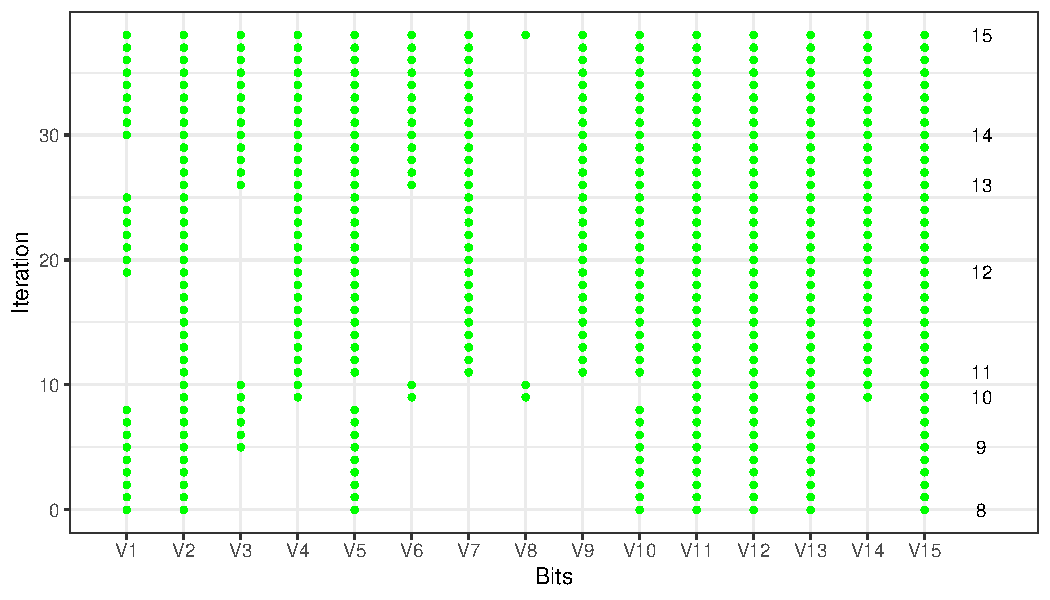
\includegraphics[width=0.7\textwidth]{figure_man/one_max_example.pdf} \\
  \begin{footnotesize}
  Green: Representation of best individual per iteration. Right scale shows fitness value of individual.  
  \end{footnotesize}
\end{figure}

\end{vbframe}



\begin{vbframe}{Example 2: Feature selection}

We consider the following simulation setting:

\begin{itemize}
\item First, we generate a $(n \times p)$ design matrix $\mathbf{X}$ by drawing $n = 1000$ samples of $p = 50$ independent normally distributed features with $\mu_j = 0$ and $\sigma_j$ varying between 1 and 5 for $j = 1, \dots, p$.
\item Then, we assume the following linear regression problem with the target variable $\mathbf{y}$ being generated as follows: 
$$
\mathbf{y} = \mathbf{X}\thetab + \epsilon
$$
with $\epsilon \sim \mathcal N(0, 1)$\\
and $\thetab$ being defined as follows
\begin{eqnarray*}
\theta_{0} &=& - 1.2 \\
\theta{j} &=& 1 \qquad \text{for } j \in \{1, 7, 13, 19, 25, 31, 37, 43\} \\
\theta{j} &=& 0 \qquad \text{else}
\end{eqnarray*}

Hence, there are 8 out of 50 equally influential features.
%<<>>=
%set.seed(123)
%X = matrix(rnorm(50000, sd = 1:5), ncol = 50, byrow = TRUE)
%@
 
%<<>>=
%vars = seq(1, 43, length = 8)
%vars
%@

%<<>>=
%y = - 1.2 + rowSums(X[, vars]) + rnorm(nrow(X), 1)
%@
\end{itemize}





\framebreak
\textbf{Aim:} Use a $(\mu + \lambda)$ selection strategy for feature selection.\\
\vspace*{0.2cm}
Our iterative algorithm with $100$ iterations is as follows:
\begin{enumerate}
\item Initialize the population and evaluate it. Therefore, encode a chromosome of an individual as a bit string of length $p$, i.e. $\textbf{z} \in \{0, 1\}^p$. Where $z_j =1$ means that variable $j$ is included in the model.
\item Apply the variation and evaluate the fitness function. As fitness function, select BIC of the model belonging to the corresponding variable configuration $\textbf{z} \in \{0, 1\}^p$.
\item Finally, use $(\mu + \lambda)$-selection strategy as the survival selection with population size of $\mu = 100$ and $\lambda =50$ offspring.
\end{enumerate}




%<<>>=
%fn = function(x) {
 % mod = lm(y ~ X[, x == 1])
  %bic = BIC(mod)
  % return(bic)
%}
%@




%\framebreak
%<<>>=
%MU = 100L # Size of the population
%LAMBDA = 50L # Number of offspring per iteration
%@

In addition:

\begin{itemize}
\item for the mutation, use bit flip with $p = 0.3$
\item for the recombination, use Uniform crossover with $p=0.5$
\end{itemize}

\lz

By exploiting \textbf{Greedy} as a selection strategy, ensure that you always choose individuals with the best fitness. 




%<<>>=
%control = initECRControl(fn, n.objectives = 1)
%control = registerECROperator(control, "mutate", mutBitflip,
%                              p = 0.3)
%control = registerECROperator(control, "selectForMating",
%                              selGreedy, n.select = LAMBDA)
%control = registerECROperator(control, "recombine",
%                              recUnifCrossover, p = 0.5)
%control = registerECROperator(control, "selectForSurvival",
%                              selGreedy)
%@



%\framebreak

\vspace{0.5cm}
\begin{center}
\begin{figure}
  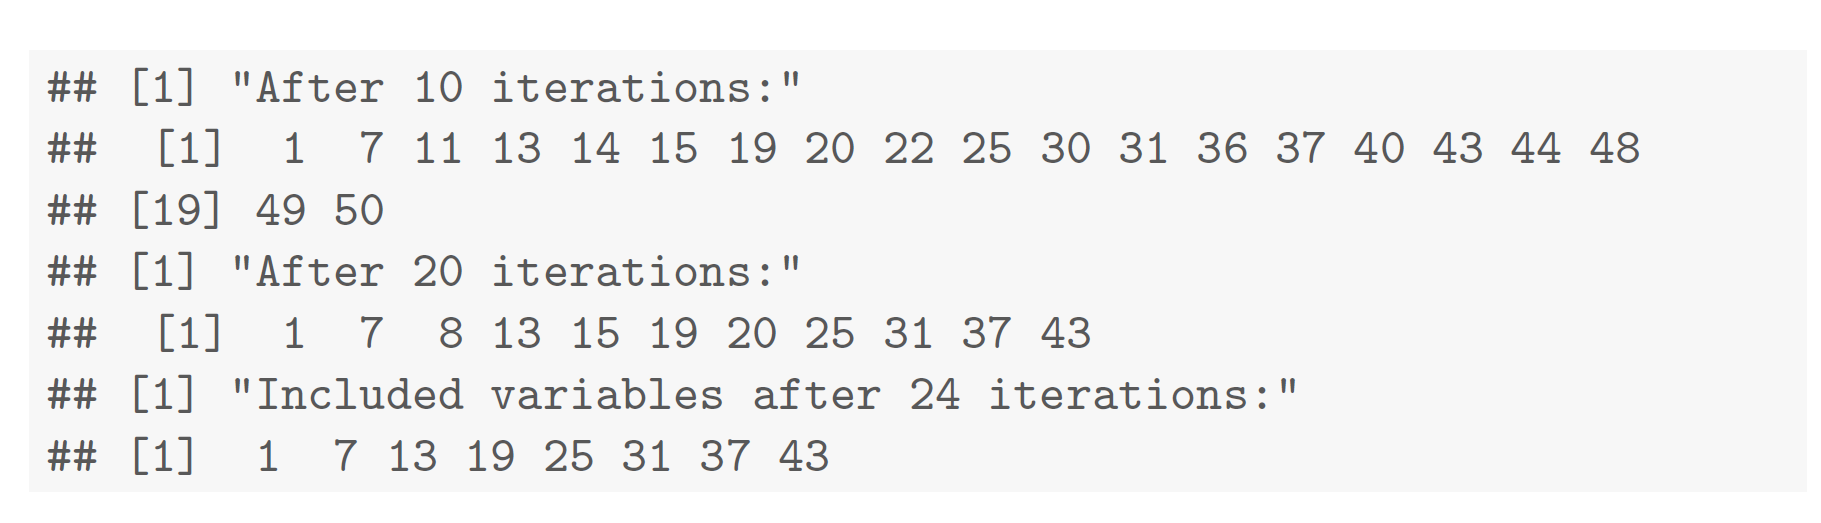
\includegraphics[height = 3cm, width = 10cm]{figure_man/example3.png}
\end{figure}
\end{center}

%<<evaluate = F>>=
%MAX.ITER = 100L # Number of iterations

%# Step 1: Initialize & rate population
%population = genBin(MU, 50)
%fitness = evaluateFitness(control, population)

%for (i in seq_len(MAX.ITER)) {
%    # Step 2: variation
%    offspring = generateOffspring(control, population, fitness,
%                                  LAMBDA)
%    fitness.o = evaluateFitness(control, offspring)

%    # Step 3: survival selection
%    sel = replaceMuPlusLambda(control, population, offspring,
%                              fitness, fitness.o)
%    population = sel$population
%    fitness = sel$fitness
%}
%@

%<<echo = F>>=
%set.seed(1234)

%MAX.ITER = 100L # Number of iterations

%# Step 1: Initialize & rate population
%population = genBin(MU, 50)
%fitness = evaluateFitness(control, population)
%bic = matrix(fitness[1, ], ncol = MU)
%best = matrix(population[[which.min(fitness)]], ncol = 50)


%for (i in seq_len(MAX.ITER)) {
%     # Step 2: variation
%    offspring = generateOffspring(control, population, fitness,
%                                  LAMBDA)
%    fitness.o = evaluateFitness(control, offspring)

%    # Step 3: survival selection
%    sel = replaceMuPlusLambda(control, population, offspring,
%                              fitness, fitness.o)
%   population = sel$population
%    fitness = sel$fitness
%    best = rbind(best, population[[which.min(fitness)]])
%    bic = rbind(bic, fitness[1, ])

%    if (i %% 10 == 0) {
%      print(paste("After", i, "iterations:"))
%      print(which(population[[1]] == 1))
%    }

%    if (all((which(population[[1]] == 1)) %in% vars)) {
%      print(paste("Included variables after", i, "iterations:"))
%      print(which(population[[1]] == 1))
%      break
%    }
%}
%@
\vspace{0.5cm}
\begin{center}
\begin{figure}
  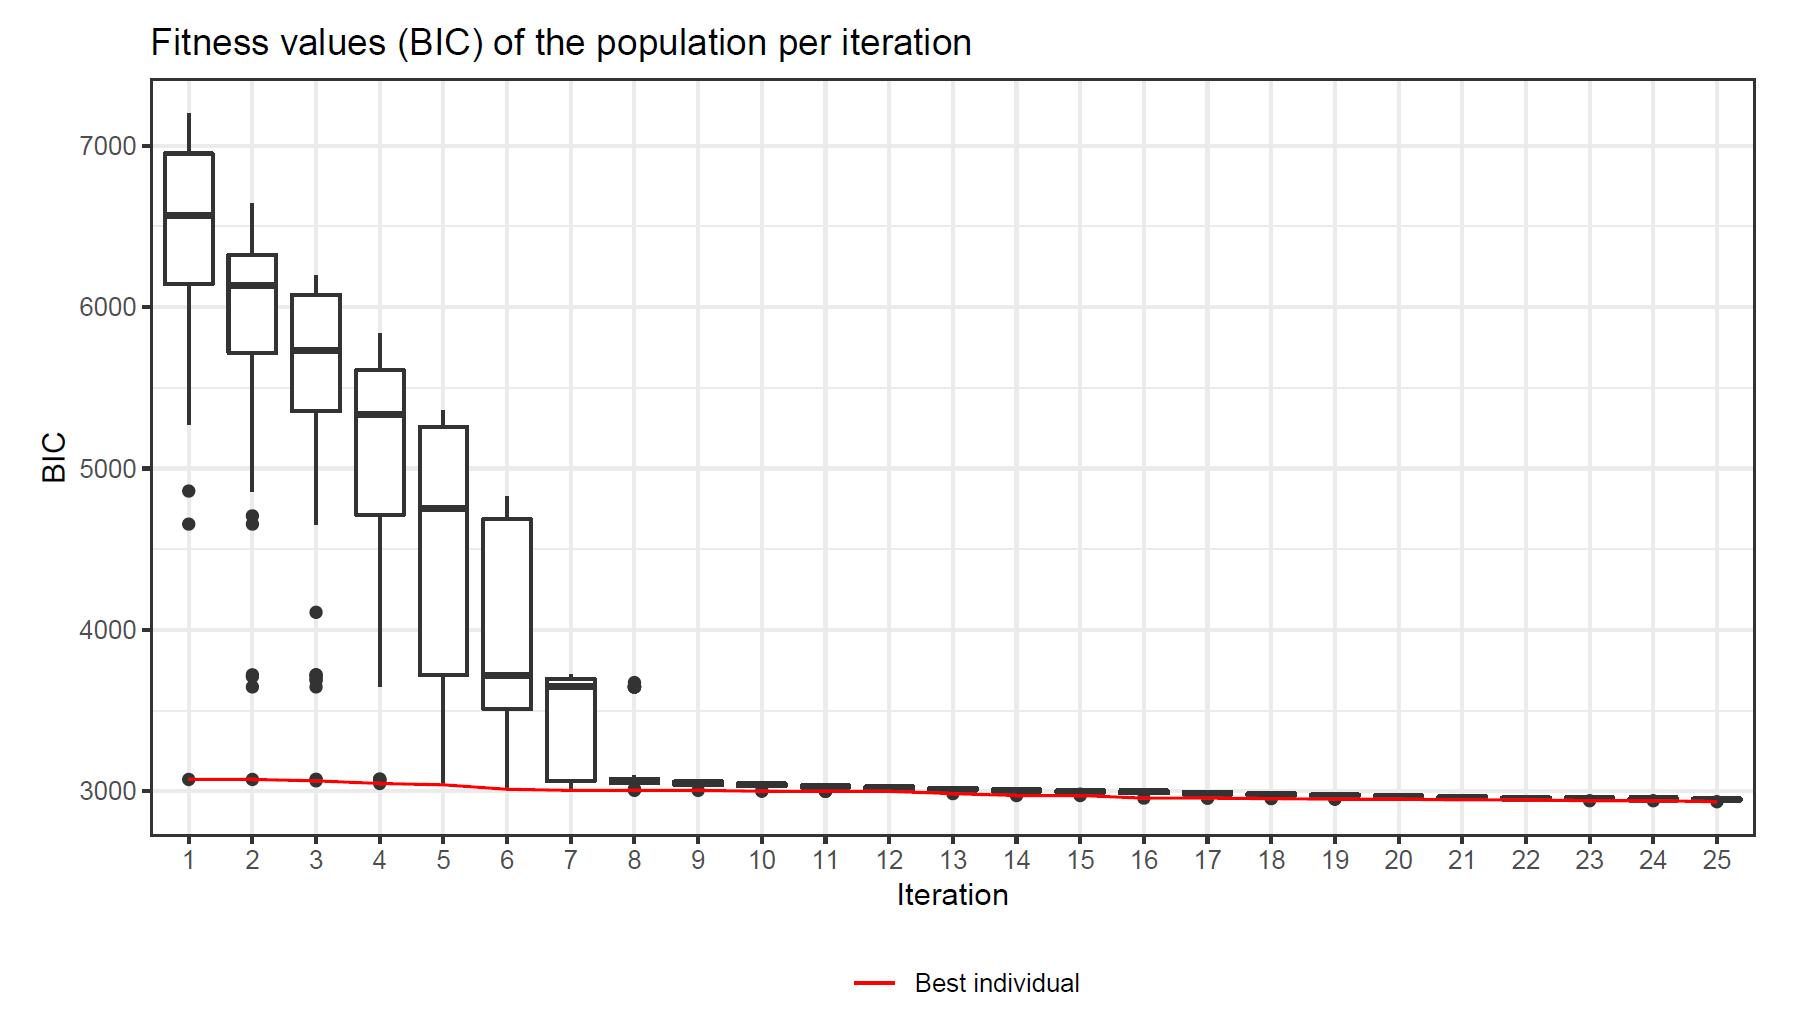
\includegraphics[height = 6cm, width = 9cm]{figure_man/var-selection1.png}
\end{figure}
\end{center}

\vspace{0.5cm}
\begin{center}
\begin{figure}
  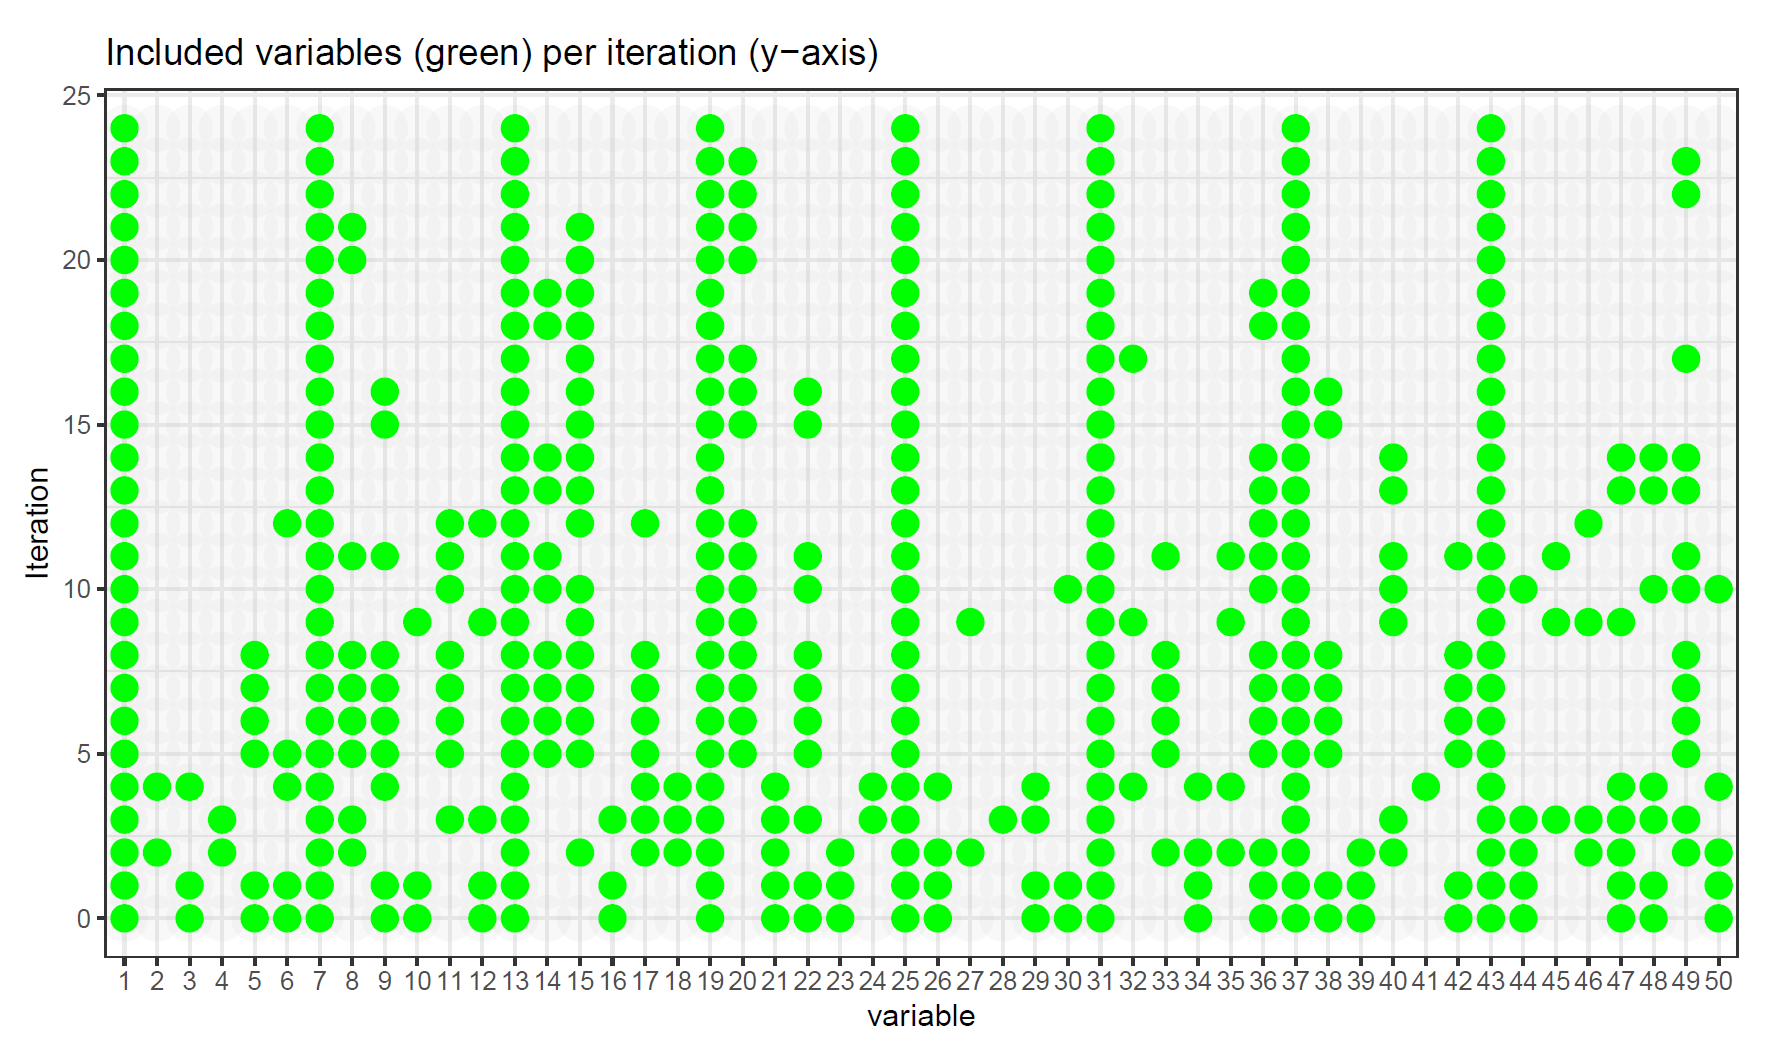
\includegraphics[height = 6cm, width = 9cm]{figure_man/var-selection2.png}
\end{figure}
\end{center}

\end{vbframe}


\begin{vbframe}{Application}

When should evolutionary algorithms be applied?

\begin{itemize}
\item Problem given by black/gray box (objective function not known or insufficiently known)
\item No problem-specific solver available
\item Problem insufficiently understood
\item No resources for developing a problem-specific solver
\item Solution with \enquote{satisfactory quality} sufficient (as a rule, EAs give no guarantee of optimality)
\end{itemize}

\end{vbframe}




% \begin{vbframe}{Anwendungen}
%
% Die Bereiche, in denen evolutionäre Algorithmen eingesetzt werden, sind nahezu unbegrenzt.
%
% \begin{itemize}
% \item Wirtschaft
% \item Forschung
% \item Kunst und Musik
% \end{itemize}
%
% \end{vbframe}



% \begin{vbframe}{8-Damen-Problem}
%
% \begin{itemize}
%   \item Acht Damen sollen so auf einem Schachbrett aufgestellt werden, dass keine
%   zwei Damen einander schlagen können. Jede Figur spielt hierbei gegeneinander.
%   \item Konkret: Keine zwei Damen dürfen auf derselben Reihe, Linie oder Diagonale stehen.
%   \item Auf klassischem 8x8-Brett gibt es 92 Lösungen die Damen aufzustellen.
% \end{itemize}
%
% \framebreak
%
% \begin{figure}
%   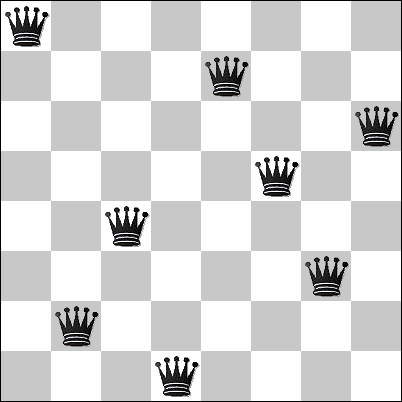
\includegraphics[width=0.5\textwidth, height=0.5\textheight]{figure_man/damen.png}
%   \caption{Eine Lösung des 8-Damen-Problems}
% \end{figure}
%
%
% \framebreak
%
% <<eval=FALSE>>=
% # create a random chessboard of size n x n
% # represent board as vectors of x and y coords
% # place queens on random coords, we even allow clashes
% # where multiple queens are on the same tile
% createRandomBoard = function(n) {
%   xs = integer(n)
%   ys = integer(n)
%   for (i in 1:n) {
%     xs[i] = sample(n, 1)
%     ys[i] = sample(n, 1)
%   }
%   list(n = n, xs = xs, ys = ys)
% }
% @
%
% \framebreak
%
% <<eval=FALSE, size='footnotesize'>>=
% # print board on console so we can understand it
% printBoard = function(b) {
%   n = b$n
%   f = matrix(".", n,n)
%   for (i in 1:n) {
%     f[b$xs[i], b$ys[i]] = i
%   }
%   for (i in 1:n) {
%     for (j in 1:n) {
%       cat(f[i,j])
%     }
%     cat("\n")
%   }
% }
% @
%
% \framebreak
%
% <<eval=FALSE, size='footnotesize'>>=
% # iterate over all queens and check conflicts
% # if a queen threatens another one, +1 penalty
% # if a queen is on top of another, +n penaly
% objective = function(b) {
%   n = b$n
%   penalty = 0
%   # check all ordered pairs of queens
%   # (yes, we then count penalties twice)
%   for (i in 1:n) {
%     for (j in setdiff(1:n, i)) {
%       x1 = b$xs[i]; y1 = b$ys[i]
%       x2 = b$xs[j]; y2 = b$ys[j]
%     cond = x1 == x2 || y1 == y2 || x1 + y1 == x2 + y2 ||
%       x1 - y1 == x2 - y2
%     [...]
% @
%
% \framebreak
%
% <<eval=FALSE, size='footnotesize'>>=
%     [...]
%     if (cond) {
%       penalty = penalty + 1
%     }
%     if (x1 == x2 && y1 == y2)
%       penalty = penalty + n
%     }
%   }
%   return(penalty)
% }
% @
%
%
% \framebreak
%
% <<eval=FALSE, size='footnotesize'>>=
%
% # do a local perturbation of the board,
% # for SA, return perturbed board
% #
% # select random queen, then:
% # method "1step": move queen 1 random step
% # to on the board (8 dirs, or even stay)
% # method: "geom": sample movement in x and y by
% # adding geometric distribution: G(0.5) - G(0.5)
% # at end: if we have left the board --> clip to board boundary
% getPerturbedBoard = function(b, op = "geom") {
%   # select random queen
%   i = sample(b$n, 1L)
%   x = b$xs[i]
%   y = b$ys[i]
%   [...]
% @
%
% \framebreak
%
% \vspace*{-0.4cm}
%
% <<eval=FALSE, size='footnotesize'>>=
%   [...]
%     # option a) move 1 random step
%   if (op == "1step") {
%     x = x + sample(c(-1,0,1), 1L)
%     y = y + sample(c(-1,0,1), 1L)
%   }
%   # option b) add geometric distruted steps
%   if (op == "geom") {
%     h = function() rgeom(1, prob = 0.5) - rgeom(1, prob = 0.5)
%     x = x + h()
%     y = y + h()
%   }
%   [...]
% }
% @
%
%
% \framebreak
%
% <<eval=FALSE, size='footnotesize'>>=
%   [...]
%   # clip to board and write x,y back to board
%   x = min(max(x, 1), b$n)
%   y = min(max(y, 1), b$n)
%   b$xs[i] = x
%   b$ys[i] = y
%   return(b)
% }
% @
%
% \framebreak
%
% <<eval=FALSE, size='footnotesize'>>=
% # simulated annealing for a starting board
% # b: board of queens
% # maxit: number of SA iterations
% # op: operator for local perturbation, see getPerturbedBoard
% # t.start: start temperature
% # t.factor: used in cooling T <- t.factor * T
% sa = function(b, maxit = 3L, op = "geom", t.start = 100,
%   t.keep = 50L, t.factor = 0.8) {
%   # init stuff
%   penalty = objective(b)
%   penalties = penalty # archive for all evals
%   temp = t.start
%   iter = 1L
%   [...]
% @
%
% \framebreak
%
% <<eval=FALSE, size='footnotesize'>>=
%   [...]
%   while(penalty > 0 && iter <= maxit) {
%     # local perturbation, evaluate it, store the eval
%     b.new = getPerturbedBoard(b, op = op)
%     p.new = objective(b.new)
%     penalties = c(penalties,p.new)
%     # compute delta diff d, and prob to accept
%     d = penalty - p.new
%     prob = exp(d / temp)
%     u = runif(1)
%     messagef("iter = %4i; cur = %4i,  new = %4i,
%         prob = %.4f,  t = %g",
%       iter, penalty, p.new, ifelse(d < 0, prob, 0) , temp)
%     # accept if we are better, or randomly if we are worse
%
%     [...]
% @
%
% \framebreak
%
% <<eval=FALSE, size='footnotesize'>>=
%     [...]
%     if (d > 0 || u < prob) {
%       b = b.new
%       penalty = p.new
%     }
%
%     # decrease temperature
%     if (iter %% t.keep == 0)
%       temp = temp * t.factor
%     iter = iter + 1L
%   }
%   list(b = b, penalty = penalty, penalties = penalties)
% }
% @
%
%
% \framebreak
%
% <<echo=FALSE, cache=TRUE>>=
% source("rsrc/sa-8queens-example/board.R")
% source("rsrc/sa-8queens-example/objective.R")
% source("rsrc/sa-8queens-example/sa.R")
% @
%
% <<message = FALSE, cache = TRUE>>=
% set.seed(5)
% b1 = createRandomBoard(8)
% printBoard(b1)
% print(objective(b1))
% @
%
% \framebreak
%
% <<message = FALSE, cache = TRUE>>=
% z = sa(b1, maxit = 2000, t.factor = 0.8, t.start = 100)
% b2 = z$b
% printBoard(b2)
% print(objective(b2))
% @
%
% \framebreak
%
% <<cache=TRUE>>=
% library(plyr)
% n = 8L
% nrep = 10L
% maxit = 10000L
%
% methods = c("random", "greedy", "sa1", "sa2", "sa3", "sa4")
% ops = c("1step",  "geom")
% reps = 1:nrep
% t.starts =  c(random = 100000, greedy = 1e-16,
%   sa1 = 100, sa2 = 100, sa3 = 10, sa4 = 1)
% t.factors = c(random = 1, greedy = 1,
%   sa1 = 0.8, sa2 = 0.7, sa3 = 0.8, sa4 = 0.8)
% grid = expand.grid(method = methods, op = ops, rep = reps)
%
% boards = lapply(reps, function(i) createRandomBoard(n = n))
% @
%
% \framebreak
%
% <<eval = FALSE, message=FALSE>>=
% for (i in seq_row(grid)) {
%   g = grid[i, ]
%   m = as.character(g$method)
%   b = boards[[g$rep]]
%   z = sa(b, maxit = maxit, op = g$op , t.start = t.starts[m],
%     t.factor = t.factors[m])
%   grid[i, "y"] = min(z$penalties)
%   grid[i, "ert"] = length(z$penalties)
% }
% grid2 = ddply(grid, c("method", "op"), summarize, ert = median(ert))
% @
%
% <<results = 'hide', echo = FALSE, eval = FALSE, message=FALSE>>=
% # library(plyr)
% # library(parallelMap)
% # parallelStartSocket(30)
% # parallelExport("grid", "t.starts", "t.factors", "n", "maxit", "rep", "boards")
% # parallelLibrary("BBmisc")
% # parallelSource(files = paste0(getwd(),c("/sa-8queens-example/board.R", "/sa-8queens-example/objective.R", "/sa-8queens-example/sa.R")))
% # z = parallelLapply(seq_row(grid), function(i) {
% #   g = grid[i, ]
% #   m = as.character(g$method)
% #   b = boards[[g$rep]]
% #   return(sa(b, maxit = maxit, op = g$op , t.start = t.starts[m], t.factor = t.factors[m]))
% # })
% # parallelStop()
% #
% # grid[, "y"] = vnapply(z, function(x) min(x$penalties))
% # grid[, "ert"] = vnapply(z, function(x) length(x$penalties))
% #
% # grid2 = ddply(grid, c("method", "op"), summarize, ert = median(ert))
% # save(grid, grid2, file = "sa-8queens-example/sa-8queens-benchmark.RData")
% @
%
% \framebreak
%
% <<echo = -1>>=
% load("rsrc/sa-8queens-example/sa-8queens-benchmark.RData")
% grid[1:12, ]
% @
%
% \framebreak
%
% <<>>=
% grid2
% @
%
% \end{vbframe}

% \section{Optimierung in R}
%
% \begin{vbframe}{Optimierung in R}
% Funktion \pkg{optim()} aus base R stellt Algorithmen für allgemeine Optimierungsprobleme bereit: \\[0.15cm]
% \begin{itemize}
% \item \textbf{BRENT:} Nur für eindimensionale Funktionen. Benutzt die Funktion \pkg{optimize()}.
%       Kann sinnvoll sein, wenn \pkg{optim()} innerhalb einer anderen Funktion aufgerufen wird.
% \item \textbf{CG:} Konjugierte Gradienten Verfahren
% % \item \textbf{Nelder-Mead Simplex:} Gut für nicht-dif'bare Funktionen, basiert nur auf Funktionsauswertungen (default)
% \item \textbf{BFGS, Quasi-Newton:} Veröffentlicht in 1970 zeitgleich durch Broyden, Fletcher, Goldfarb and Shanno
% % \item \textbf{SANN:} Stochastisches Simulated Annealing
% \end{itemize}
% \framebreak
% <<eval=FALSE>>=
% # Grundlegender Aufruf:
% optim(par, fn, gr, method, lower, upper, control)
% @
% \begin{itemize}
% \item \textbf{par} Startwerte der zu optimierenden Parameter
% \item \textbf{fn} (Objective) Function, die optimiert (default: minimiert) werden soll
% \item \textbf{gr} Gradient/Ableitung bei entsprechender Methode
% \item \textbf{method} Optimierungsmethode (siehe oben)
% \item \textbf{lower/upper} Grenzen für Optimierung (L-BFGS-B)
% \item \textbf{control} Liste von Kontrollparametern
% \end{itemize}
% \end{vbframe}



\endlecture
\end{document}